\documentclass{standalone}

\usepackage{tikz}
\usetikzlibrary{shapes}
\begin{document}


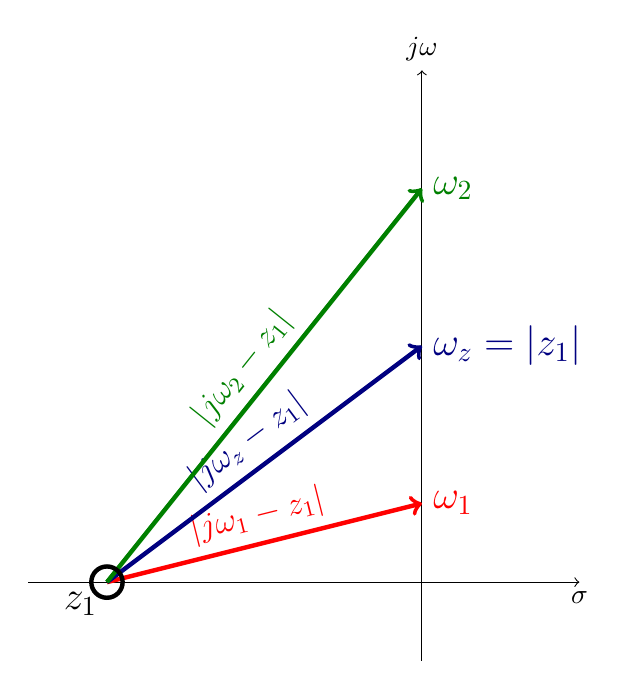
\begin{tikzpicture}
  \draw[->] (-5,0) -- (2,0) node[below] {$\sigma$};
  \draw[->] (0,-1) -- (0,6.5) node[above] {$j\omega$};

  \draw[->,ultra thick, color=red] (-4,0) -- node[midway, sloped, above, font =\large] {$|j\omega_1 - z_1|$} (0,1) node[right, font = \Large] {$\omega_1$};
  \draw[->,ultra thick, color=blue!50!black] (-4,0) -- node[midway, sloped, above, font =\large] {$|j\omega_z - z_1|$} (0,3) node[right, font = \Large] {$\omega_z = |z_1|$};
  \draw[->,ultra thick, color=green!50!black] (-4,0) -- node[midway, sloped, above, font =\large] {$|j\omega_2 - z_1|$} (0,5) node[right, font = \Large] {$\omega_2$};

  \node[circle, ultra thick, color = black, draw, inner sep=4pt] at (-4,0) {};
  \node[below left, font = \Large] at (-4, 0) {$z_1$};

\end{tikzpicture}

\end{document}
